% This file was created (at least in part) by the script ParseMdtoLatex by Louis du Plessis
% (Available from https://github.com/taming-the-beast)

\documentclass[11pt]{article}
\usepackage[]{authblk}
\usepackage{graphicx}
\usepackage{color}
\usepackage{longtable}
\usepackage{hanging}
\usepackage{indentfirst}
\usepackage{setspace}
\usepackage{enumitem}
\usepackage{verbatim}
\usepackage{upgreek}
\usepackage{framed}
\usepackage{ textcomp }
\usepackage{url}
\usepackage{soul}
\usepackage{amsmath, amsfonts,amssymb,mathrsfs}
\usepackage{fancyhdr}
\usepackage[compact]{titlesec}
\usepackage[T1]{fontenc}
\usepackage{lmodern}

\usepackage[backend=bibtex,hyperref=true,citestyle=authoryear,bibstyle=authortitle,firstinits=true,terseinits=true,doi=false,url=false,eprint=false,maxbibnames=10,maxcitenames=2]{biblatex}
\DeclareCiteCommand{\cite}
  {\usebibmacro{prenote}}
  {\usebibmacro{citeindex}%
   \printtext[bibhyperref]{\usebibmacro{cite}}}
  {\multicitedelim}
  {\usebibmacro{postnote}}

\DeclareCiteCommand*{\cite}
  {\usebibmacro{prenote}}
  {\usebibmacro{citeindex}%
   \printtext[bibhyperref]{\usebibmacro{citeyear}}}
  {\multicitedelim}
  {\usebibmacro{postnote}}

\DeclareCiteCommand{\parencite}[\mkbibparens]
  {\usebibmacro{prenote}}
  {\usebibmacro{citeindex}%
    \printtext[bibhyperref]{\usebibmacro{cite}}}
  {\multicitedelim}
  {\usebibmacro{postnote}}

\DeclareCiteCommand*{\parencite}[\mkbibparens]
  {\usebibmacro{prenote}}
  {\usebibmacro{citeindex}%
    \printtext[bibhyperref]{\usebibmacro{citeyear}}}
  {\multicitedelim}
  {\usebibmacro{postnote}}

\DeclareCiteCommand{\footcite}[\mkbibfootnote]
  {\usebibmacro{prenote}}
  {\usebibmacro{citeindex}%
  \printtext[bibhyperref]{ \usebibmacro{cite}}}
  {\multicitedelim}
  {\usebibmacro{postnote}}

\DeclareCiteCommand{\footcitetext}[\mkbibfootnotetext]
  {\usebibmacro{prenote}}
  {\usebibmacro{citeindex}%
   \printtext[bibhyperref]{\usebibmacro{cite}}}
  {\multicitedelim}
  {\usebibmacro{postnote}}

\DeclareCiteCommand{\textcite}
  {\boolfalse{cbx:parens}}
  {\usebibmacro{citeindex}%
   \printtext[bibhyperref]{\usebibmacro{textcite}}}
  {\ifbool{cbx:parens}
     {\bibcloseparen\global\boolfalse{cbx:parens}}
     {}%
   \multicitedelim}
  {\usebibmacro{textcite:postnote}}

\newcommand{\citep}{\parencite}
\newcommand{\citet}{\textcite}
\defbibheading{relevref}[\refname]{\section*{Relevant References}}

\renewcommand{\postnotedelim}{\iffieldpages{postnote}{\addcolon}{\addcomma\space}} 
\DeclareFieldFormat{postnote}{#1} 

\DeclareFieldFormat[article, inbook, incollection, inproceedings, patent, thesis, unpublished]{title}{#1}
\DeclareFieldFormat[article, inbook, incollection, inproceedings, patent, thesis, unpublished]{journaltitle}{\mkbibemph{#1}\nopunct}
\DeclareFieldFormat[article, inbook, incollection, inproceedings, patent, thesis, unpublished]{volume}{{#1}\addcolon} %puts volume number in parens
%\DeclareFieldFormat[article, inbook, incollection, inproceedings, patent, thesis, unpublished]{year}{\mkbibparens{#1}\nopunct} %puts year in parens

\DeclareFieldFormat[article, incollection, patent, thesis, unpublished]{pages}{{\nopp#1}}

\DeclareFieldFormat{sentencecase}{\MakeSentenceCase{#1}}

\renewbibmacro*{title}{%
  \ifthenelse{\iffieldundef{title}\AND\iffieldundef{subtitle}}
    {}
    {\ifthenelse{\ifentrytype{article}\OR\ifentrytype{inbook}%
      \OR\ifentrytype{incollection}\OR\ifentrytype{inproceedings}%
      \OR\ifentrytype{inreference}}
      {\printtext[title]{%
        \printfield[sentencecase]{title}%
        \setunit{\subtitlepunct}%
        \printfield[sentencecase]{subtitle}}}%
      {\printtext[title]{%
        \printfield[titlecase]{title}%
        \setunit{\subtitlepunct}%
        \printfield[titlecase]{subtitle}}}%
     \newunit}%
  \printfield{titleaddon}}

\DefineBibliographyStrings{english}{% various adjustments to common bib entry strings
urlseen = {Accessed:},% What goes in front of the date a URL was accessed/retrieved etc.
editor = {(Ed)},%Ed – no dot, in brackets
editors = {(Eds)},% Eds – no dot, in brackets
byeditor = {(Ed.)}}% ‘Edited by’ for edited works

\DeclareNameAlias{default}{last-first}

\renewbibmacro{in:}{}

\renewbibmacro{publisher+location+date}{
  \iflistundef{publisher}
    {}
    {\printlist{publisher}%
       {\addcomma\space}%
      \iflistundef{location}
        {}
        {\printlist{location}}%
    }
}

\DeclareBibliographyDriver{article}{%
\usebibmacro{bibindex}%
\usebibmacro{begentry}%
\usebibmacro{author/translator+others}%
\newunit\newblock
\printfield{year}%
\setunit{\labelnamepunct}\newblock
\usebibmacro{title}%
\newunit
\printlist{language}%
\newunit\newblock
\usebibmacro{byauthor}%
\newunit\newblock
\usebibmacro{bytranslator+others}%
\newunit\newblock
\printfield{version}%
\newunit\newblock
%\usebibmacro{in:}% %mit in:
\usebibmacro{journal}%
\newunit\newblock
\printfield{volume}%
\newunit\newblock
\usebibmacro{byeditor+others}%
\newunit\newblock
\usebibmacro{note+pages}%
\newunit\newblock
\iftoggle{bbx:isbn}
{}%
\newunit\newblock
\usebibmacro{doi+eprint+url}%
\newunit\newblock
\usebibmacro{addendum+pubstate}%
\newunit\newblock
\usebibmacro{pageref}%
\usebibmacro{finentry}}

\DeclareBibliographyDriver{inproceedings}{%
\usebibmacro{bibindex}%
\usebibmacro{begentry}%
\usebibmacro{author/translator+others}%
\newunit\newblock
\printfield{year}%
\setunit{\labelnamepunct}\newblock
\usebibmacro{title}%
\newunit
\printlist{language}%
\newunit\newblock
\usebibmacro{byauthor}%
\newunit\newblock
\usebibmacro{bytranslator+others}%
\newunit\newblock
\printfield{version}%
\newunit\newblock
%\usebibmacro{in:}% %mit in:
\usebibmacro{booktitle}%
\newunit\newblock
\printfield{volume}%
\newunit\newblock
\usebibmacro{byeditor+others}%
\newunit\newblock
\usebibmacro{publisher+location+date}%
\newunit\newblock
\usebibmacro{note+pages}%
\newunit\newblock
\usebibmacro{pageref}%
\usebibmacro{finentry}}

\DeclareBibliographyDriver{book}{%
\usebibmacro{bibindex}%
\usebibmacro{begentry}%
\usebibmacro{author/translator+others}%
\newunit\newblock
\printfield{year}%
\setunit{\labelnamepunct}\newblock
\usebibmacro{title}%
\newunit
\printlist{language}%
\newunit\newblock
\usebibmacro{byauthor}%
\newunit\newblock
\usebibmacro{bytranslator+others}%
\newunit\newblock
%\usebibmacro{in:}% %mit in:
\usebibmacro{booktitle}%
\newunit\newblock
\printfield{volume}%
\newunit\newblock
\usebibmacro{publisher+location+date}%
\newunit\newblock
\usebibmacro{note+pages}%
\newunit\newblock
\usebibmacro{pageref}%
\usebibmacro{finentry}}





\setlength{\evensidemargin}{0in}
\setlength{\headheight}{0in}
\setlength{\headsep}{0in}
\setlength{\oddsidemargin}{-0.25in}
\setlength{\paperheight}{11in}
\setlength{\paperwidth}{8.5in}
\setlength{\tabcolsep}{0in}
\setlength{\textheight}{9in}
\setlength{\textwidth}{7in}
\setlength{\topmargin}{0in}
\setlength{\topskip}{0in}
\setlength{\voffset}{0in}
\parskip = 0.15in
\pagestyle{plain}
\setlength{\parindent}{0cm}

\definecolor{citescol}{RGB}{194,101,1}
\definecolor{urlscol}{RGB}{0,150,206}
\definecolor{linkscol}{RGB}{149,0,207}
\definecolor{mycol}{RGB}{25,23,191}
\definecolor{outputcol}{RGB}{34,139,34}
\definecolor{tcol}{RGB}{165,0,14}


\DeclareMathAlphabet{\msfsl}{T1}{cmr}{m}{it}
\DeclareMathAlphabet{\msyf}{OMX}{pcr}{m}{it}
\newcommand{\alf}{\upalpha}
\newcommand{\hilight}[1]{\colorbox{yellow}{#1}}

\newcommand{\levelone}[1]{
\bigskip
\noindent{\LARGE{\textsc{#1}}}
\vspace {0.05in}
}

\newcommand{\leveltwo}[1]{
\bigskip
\noindent{\Large{\textit{#1}}}
\vspace {-1mm}
}

\newcommand{\descriptionhead}[1]{
\noindent{\textcolor{mycol}{\textbf{\textit{#1}}}}\\ \vspace{-7mm}
}

\newcommand{\dhead}[1]{
\noindent{\textbf{\textit{#1 --}}}
}



\newcommand{\exs}[1]{
\vspace{-4mm}
\begin{itemize}
\item #1 \\ \vspace{-8mm}
\end{itemize}
}

\newcommand{\nbo}[1]{{\color{red}{#1}}}


\newcommand{\stepbullet}{\noindent \textbullet \ }
\newcommand{\mi}[1]{\textbf{\textit{#1}}}


\newcommand{\levelthree}[1]{\textit{#1 --}}


%\bibliographystyle{apalike}
%\bibpunct[; ]{(}{)}{;}{a}{,}{;}


\usepackage[breaklinks]{hyperref}
\usepackage[all]{hypcap}
\hypersetup{colorlinks=true,linkcolor=linkscol,citecolor=citescol,urlcolor=urlscol}


\newcommand{\R}{\texttt{R} }
\newcommand{\TESS}{\texttt{TESS}}
\newcommand{\PBD}{\texttt{PBD}}
\newcommand{\DDD}{\texttt{DDD}}
\newcommand{\Laser}{\texttt{laser}}
\newcommand{\TreePar}{\texttt{TreePar}}
\newcommand{\diversitree}{\texttt{diversitree}}
\newcommand{\RevBayes}{\texttt{RevBayes}}
\newcommand{\Rev}{\texttt{Rev}}
\newcommand{\MrBayes}{\texttt{MrBayes}}
\newcommand{\BEAST}{\texttt{BEAST}}
\newcommand{\PhyloBayes}{\texttt{PhyloBayes}}
\newcommand{\PAML}{\texttt{PAML}}

\let\otheriint\iint
\let\iint\relax
\usepackage{ wasysym }

\usepackage{framed}
\usepackage[]{listings}
%\usepackage{fontspec}
\usepackage{placeins}
\usepackage{epstopdf}

\lstset{breaklines=true}

\definecolor{shadecolor}{RGB}{194,225,255}

\setlength{\tabcolsep}{5pt}
\setlength{\topmargin}{-0.4in}
\setlength{\headheight}{14.5pt}
\pagestyle{fancy}

\newcommand{\taha}[1]{{\textcolor{red}{[TAH comment: #1]}}} % TAH comment

\titlespacing{\section}{0pt}{*0}{*0}
\titlespacing{\subsection}{0pt}{*0}{*0}
\titlespacing{\subsubsection}{0pt}{*0}{*0}

\titleformat{\section}
  {\normalfont\Large\bfseries\color{mycol}}
  {\thesection}{1em}{}

\titleformat{\subsection}
  {\normalfont\large\bfseries\color{mycol}}
  {\thesubsection}{1em}{}

\titleformat{\subsubsection}
  {\normalfont\bfseries\color{mycol}}
  {\thesubsubsection}{1em}{}

% command for MrBayes command-line step
\newcommand{\cl}[1]{{\texttt{\textbf{#1}}}}

\newcommand{\colx}[1]{{\textcolor{tcol}{#1}}}

\newcommand{\mbcl}[1]{\exs{\cl{MrBayes > {#1}}}}

\newcommand{\rbprmt}{RevBayes > } 
\newcommand{\rbcl}[1]{\exs{\cl{\rbprmt{#1}}}}
\newcommand{\rbout}[1]{\exs{\cl{\textcolor{outputcol}{#1}}}}
\newcommand{\rbdn}{{\Large \symbol{126}}} % This makes a copy/pasteable tilde
\newcommand{\rbclml}[1]{\exs{\cl{\ \ \ \ \ \ \ \ \ \ \ {#1}}}}

% text box settings
% requires compiling w/ XeLaTeX
%\newfontfamily\listingsfont[Scale=1.0]{Courier New}
%\lstset{basicstyle=\listingsfont, columns=texcl}
%\defaultfontfeatures{Mapping=tex-text}


\makeatletter
\lst@CCPutMacro\lst@ProcessOther {"2D}{\lst@ttfamily{-{}}{-{}}}
\@empty\z@\@empty
\makeatother



% Add your bibtex library here
\addbibresource{master-refs}


%%%%%%%%%%%%%%%%%%%%
% Do NOT edit this %
%%%%%%%%%%%%%%%%%%%%
\begin{document}
\renewcommand{\headrulewidth}{0.5pt}
\headsep = 20pt
\lhead{ }
\rhead{\textsc {BEAST v2 Tutorial}}
\thispagestyle{plain}


%%%%%%%%%%%%%%%%%%
% Tutorial title %
%%%%%%%%%%%%%%%%%%
\begin{center}

	% Enter the name of your tutorial here
	\textbf{\LARGE Structured coalescent}\\\vspace{2mm}

	% Enter a short description of your tutorial here
	\textbf{\textcolor{mycol}{\Large Population structure using MultiTypeTree}}\\

	\vspace{4mm}

	% Enter the names of all the authors here
	{\Large {\em Nicola F. Müller and Tim Vaughan}}
\end{center}


%%%%%%%%%%%%%%%%%
% Tutorial body %
%%%%%%%%%%%%%%%%%

\section{Background}\label{background}

Population dynamics can influence the shape of a tree. Another thing
that has strong influence on the shape of the tree is structure in a
population. This is the case as soon as sequences do not mix well,
i.e.~they cluster together. One cause of this clustering is due to
geography. Samples may not have been taken from the same geographic
region, leading to clustering of samples from the same region. This
clustering of samples can bias the estimation of parameters. The
extension of the classic coalescent to the structured coalescent by
allowing for migration between regions is trying to circumvent this by
allowing individual regions to have distinct coalescent rates and by
allowing migration between those regions.

\section{Programs used in this
Exercise}\label{programs-used-in-this-exercise}

\subsubsection{BEAST - Bayesian Evolutionary Analysis Sampling
Trees}\label{beast---bayesian-evolutionary-analysis-sampling-trees}

BEAST version 2.4.2 \citep{Bouckaert2014}.

\subsubsection{BEAUti - Bayesian Evolutionary Analysis
Utility}\label{beauti---bayesian-evolutionary-analysis-utility}

GUI to create \lstinline!*.xml! for BEAST2.

\subsubsection{Tracer}\label{tracer}

Tracer (\url{http://tree.bio.ed.ac.uk/software/tracer}) is used to
summarize the posterior estimates of the various parameters sampled by
the Markov Chain. It includes code to analyze estimates of past
population dynamics from \lstinline!*.log! files and \lstinline!*.trees!
files. It is mainly used for visual inspection and assessment of
convergence of MCMC runs. It helps to quickly view median estimate and
95\% credible intervals (which approximate the 95\% highest posterior
density intervals) of the parameters, and calculates the effective
sample sizes (ESS) of parameters. It also helps to visualize potential
parameter correlations.

\subsubsection{TreeAnnotator}\label{treeannotator}

TreeAnnotator is a program that comes with BEAST2. It allows to
summarize the analysis of sampled trees.

\section{Practical: MultiTypeTree}\label{practical-multitypetree}

In this tutorial we will estimate migration rates, effective population
sizes and locations of internal nodes using the structured coalescent
implemented in BEAST2, MultiTypeTree \citep{Vaughan2014}.

The aim is to:

\begin{itemize}

\item
  Learn how to infer structure from trees with sampling location
\item
  Get to know how to choose the set-up of such an analysis
\item
  Get to know the advantages and disadvantages of working with
  structured trees
\end{itemize}

\subsection{The Data}\label{the-data}

The dataset consists of 60 Influenza A/H3N2 sequences sampled in Hong
Kong and in New Zealand between 2001 and 2005. South-East Asia has been
hypothesized to be a global source location of seasonal Influenza, while
more temperate regions such as New Zealand are assumed to be global
sinks \citep{Rambaut2008,Russell2008,Lemey2014}, meaning that Influenza
strains are more likely to migrate from the tropic to the temperate
regions then vice versa. We want to see if we can infer this source-sink
dynamic from sequence data using the structured coalescent.

\subsection{Creating the Analysis File with
BEAUti}\label{creating-the-analysis-file-with-beauti}

We will use BEAUti to generate the input XML for BEAST2 from the
sequence alignment.

\subsubsection{Install BEAST 2 Plug-Ins}\label{install-beast-2-plug-ins}

The packages MultiTypeTree is not implemented in the core of BEAST, but
has to be installed (Figure \protect\hyperlink{fig:install_mtt}{1}).

\begin{figure}
    \centering
    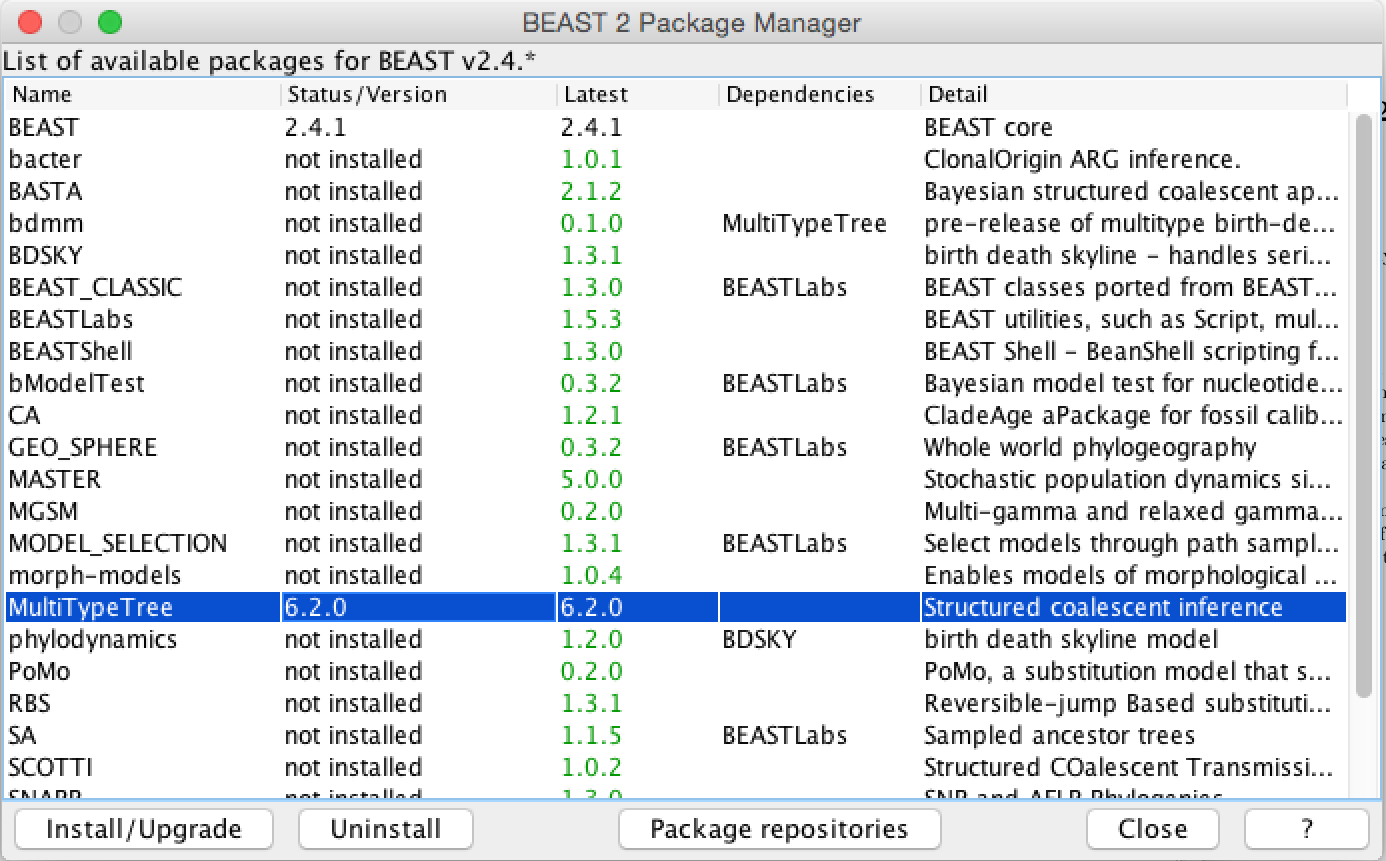
\includegraphics[width=0.500000\textwidth]{figures/install_mtt.png}
    \caption{Install MultiTypeTree.}
    \label{fig:install_mtt}
\end{figure}

To be able to make \lstinline!.xml!'s for MultiTypeTree, we have to load
the MultiTypeTree template \lstinline!File > Template > MultiTypeTree!.
This template allows to specify additional things, such as sampling
location, which one can not specify using the standard interface, as
well as parameters such as the migration rates. After setting the
template, we can load the alignment of the H3N2 data
\lstinline!File > Add Alignment!. Since the sequences were sampled
through time, we have to specify the sampling dates. These are included
in the sequence names. To set the sampling dates, go to \textbf{Tip
Dates}, guess them by splitting after the ``\_" and then choose the last
group. There are two different ways in how BEAST can interpret sampling
dates. They are labeled as \textbf{Since some time in the past} and
\textbf{Before the present}. The easiest way to check if you have used
the correct one is by checking \lstinline!Height!. If the setup is
correct, the sequences sampled the most recently (i.e.~2005.66) should
have a Height of 0 while all other tips should be larger then 0 (Figure
\protect\hyperlink{fig:sampling_dates}{2}).

\begin{figure}
    \centering
    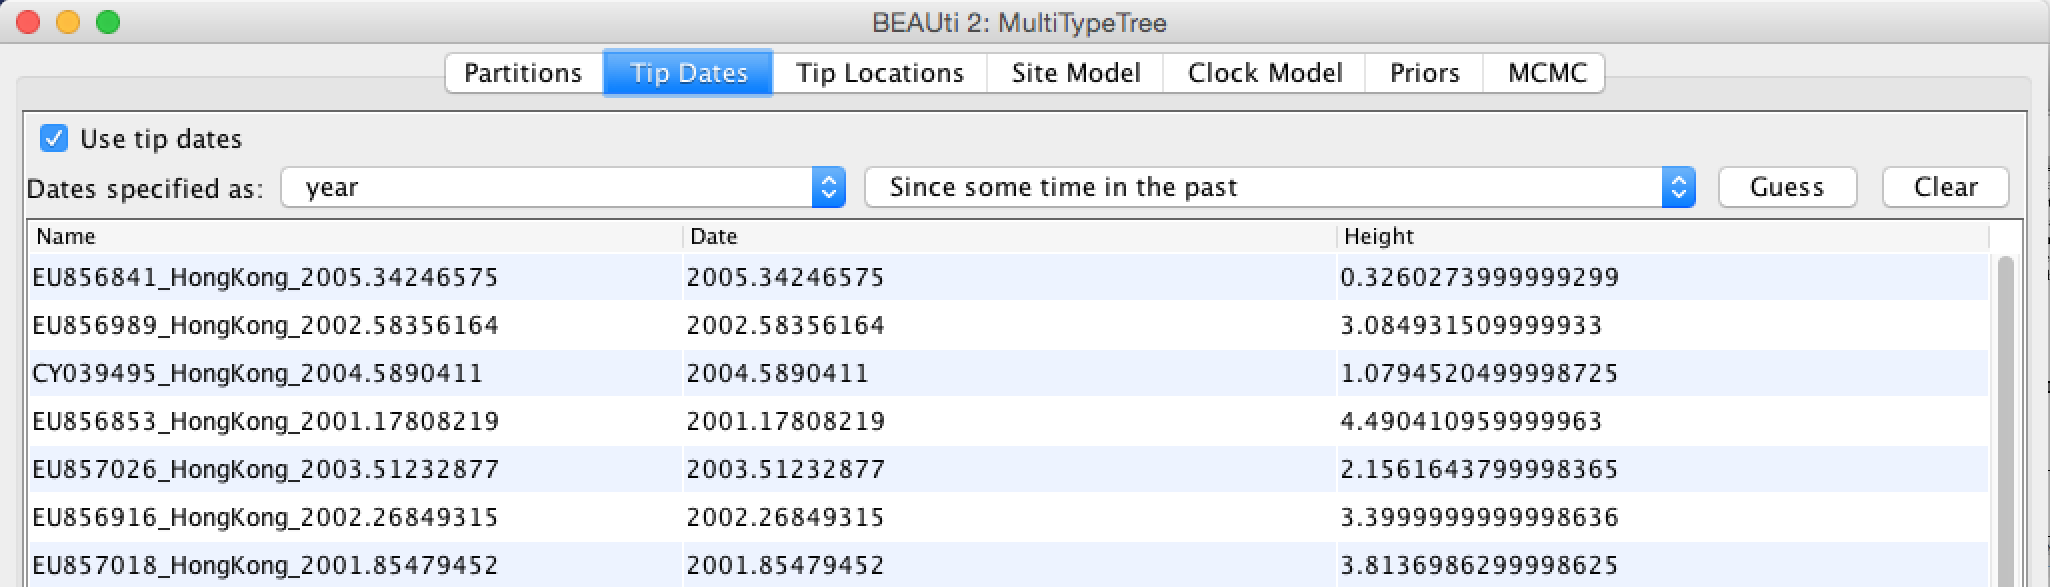
\includegraphics[max width=\textwidth, max height=0.9\textheight]{figures/dates.png}
    \caption{Sampling dates.}
    \label{fig:sampling_dates}
\end{figure}

The main contrast in the setup to previous analyses is that we include
additional information about the sampling location of sequences.
Sequences were taken from patients in Hong Kong and New Zealand. We can
specify these sampling locations by going to \textbf{Tip Locations} in
BEAUti and guessing the locations. Use here the second group after
splitting the names on the character ``\_``. After guessing the tip
locations, the column \textbf{Location} should contain the entries Hong
Kong and New Zealand (Figure
\protect\hyperlink{fig:sampling_locations}{3}).

\begin{figure}
    \centering
    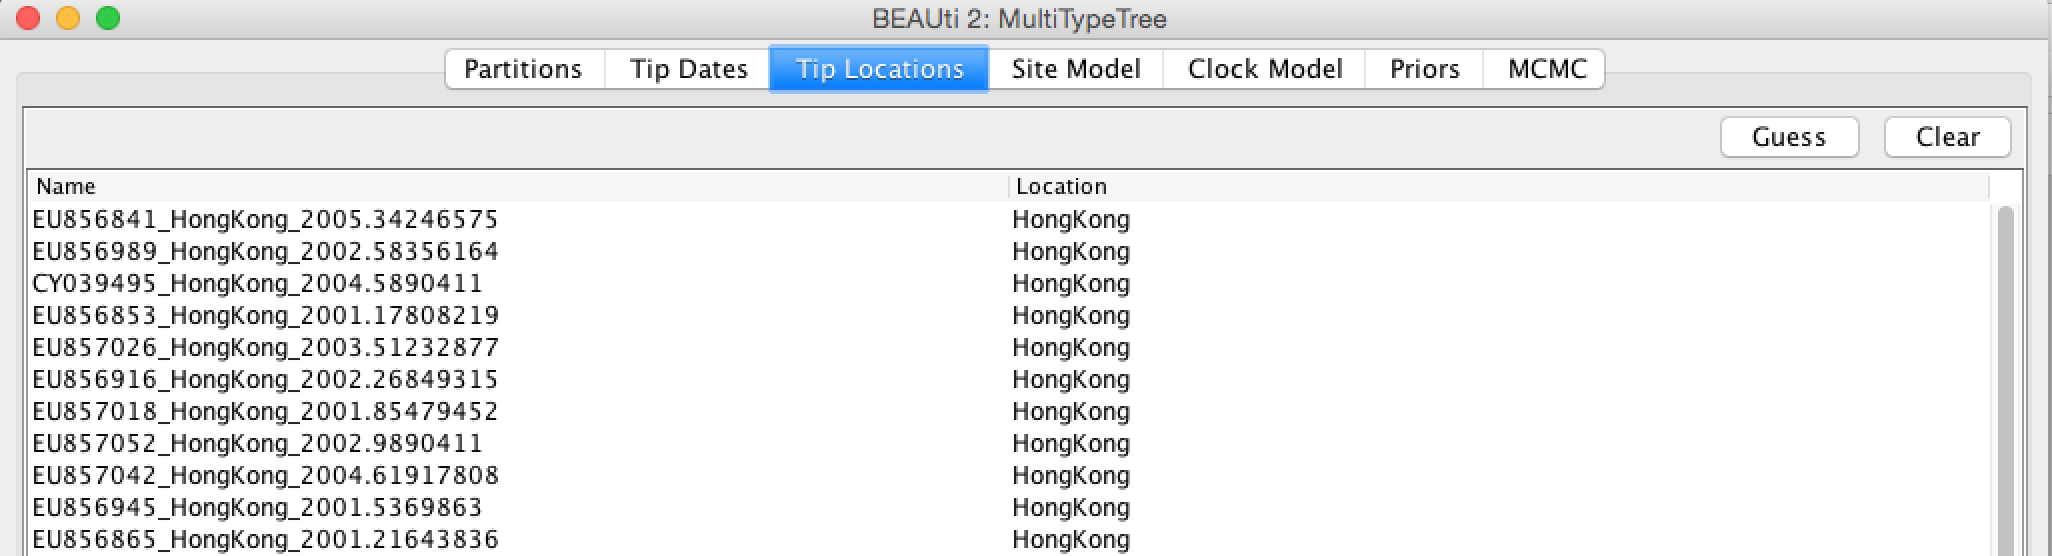
\includegraphics[max width=\textwidth, max height=0.9\textheight]{figures/locations.png}
    \caption{Sampling locations.}
    \label{fig:sampling_locations}
\end{figure}

For this analysis, we will be using the HKY model. The HKY model infers
different rates for transversion and transition. Transition being the
change within purines (\textbf{A} and \textbf{G}) and pyrimidines
(\textbf{T} and \textbf{C}) and transversion being the change among
those groups.

We also want to allow for heterogeneity between sites, which we can do
by setting the \textbf{Gamma Category Count} to a value greater than 0
(normally between 4 and 6) and ticking the \textbf{estimate} box for the
shape parameter (Figure \protect\hyperlink{fig:hky}{4}).

\begin{figure}
    \centering
    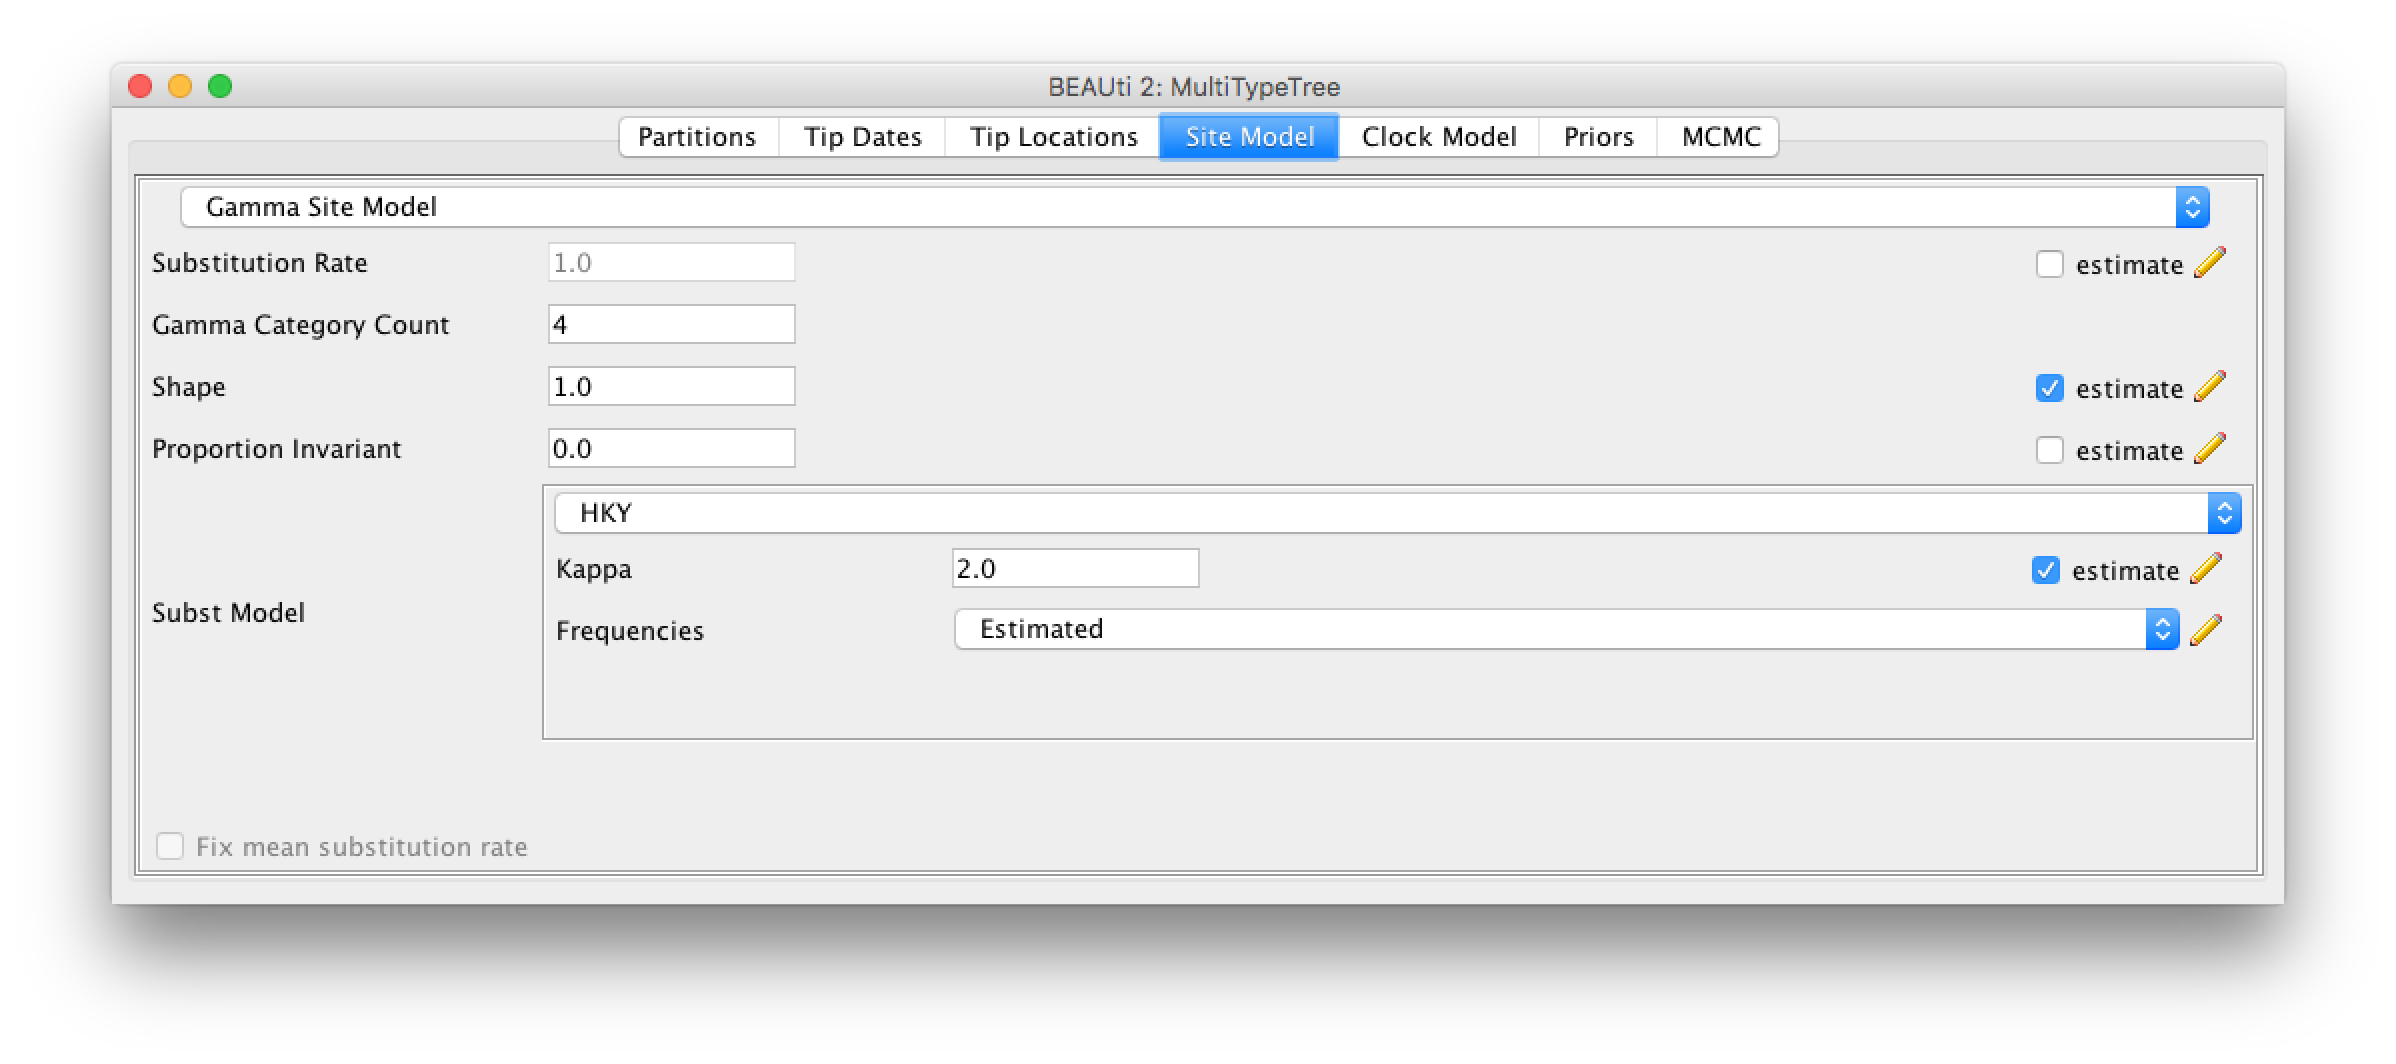
\includegraphics[max width=\textwidth, max height=0.9\textheight]{figures/choose_hky.png}
    \caption{Setup of the site model.}
    \label{fig:hky}
\end{figure}

To speed up convergence, we leave the branch model on the Strict Clock
model and set a different value for the clock rate (default is 1). A
value of 0.005 substitutions * site$^{-1}$ * year$^{-1}$ is closer to
the truth.

Since we have more than one deme (Hong Kong and New Zealand), we can
estimate the effective population size of those two demes separately.
Additionally, these demes are connected, so we can (or need to) allow
for migration between them. By default, the migration rates and
population sizes are not estimated. To change this, we have to go to the
Priors setting. There, we have to check the two \textbf{estimate} boxes
for the population sizes and the migration rates.

After checking those two boxes, there will be two new fields appearing,
where we can set the priors for the population sizes and the migration
rates. Since we know the time scale of our data (few years), we can
choose a proper prior for the migration rates, like an exponential prior
distribution with mean 1.\\
Figure \protect\hyperlink{fig:est_migrates}{5} shows the final setup for
the priors.

\begin{figure}
    \centering
    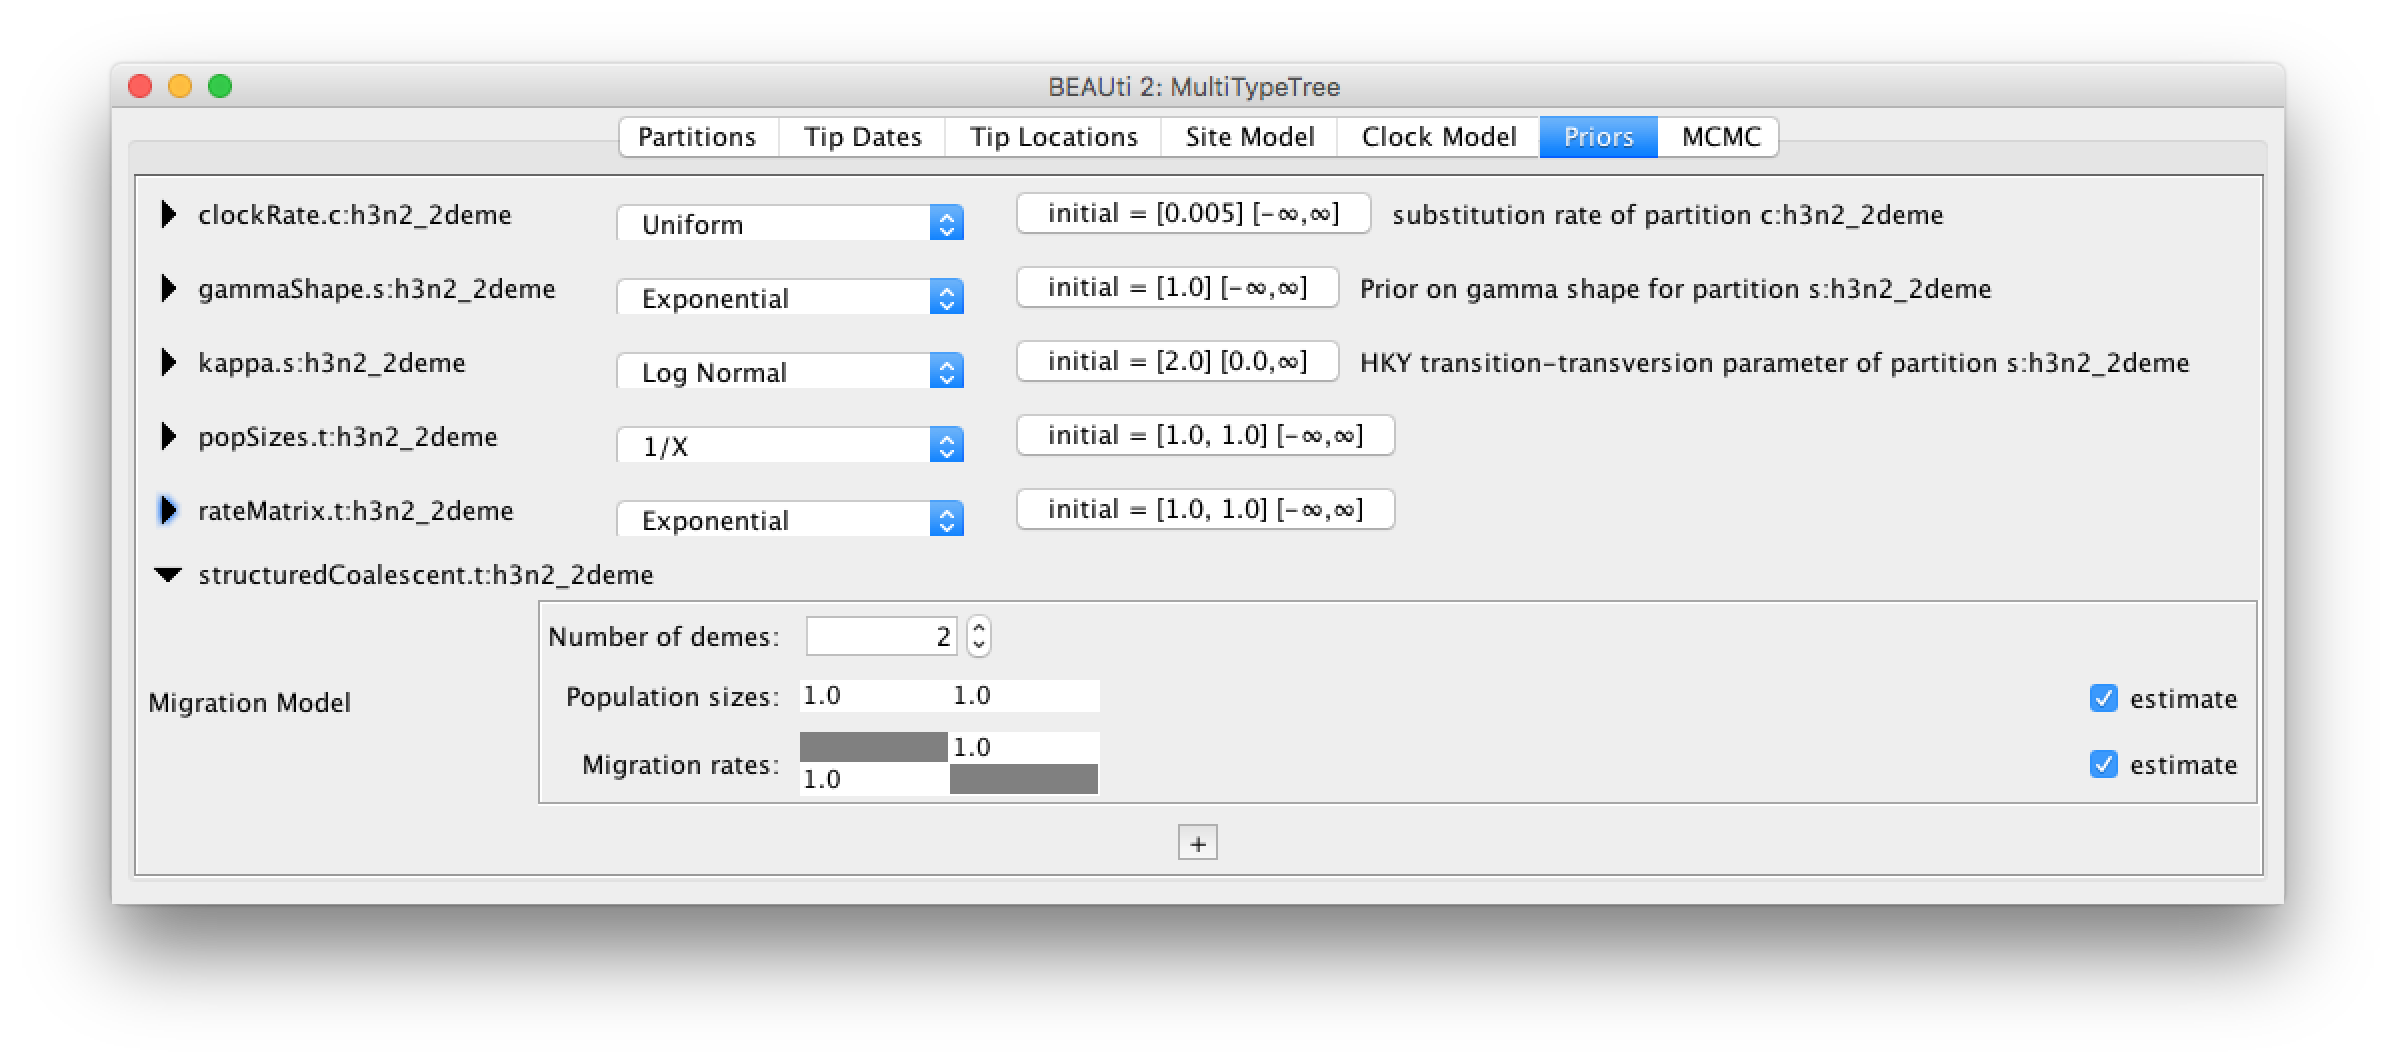
\includegraphics[max width=\textwidth, max height=0.9\textheight]{figures/estimate_migration.png}
    \caption{Check the boxes that say estimate for the population size and the migration rates and change it to an exponential prior with mean 1.}
    \label{fig:est_migrates}
\end{figure}

The rest of the settings we can leave as they are.

After saving, we get an \lstinline!*.xml!, which we can use in BEAST2.
The run will take a bit of time. If the MultiTypeTree run consumes too
much CPU power, you can just close it and then use the ``pre-cooked''
\lstinline!*.log! and \lstinline!*.trees! files later instead.

\subsubsection{Analysis of the MultiTypeTree
run}\label{analysis-of-the-multitypetree-run}

Load the \lstinline!*.log! files into tracer. First, we should check
that the run has converged by looking at the ESS values. If all ESS
values are above 200, we should be on the safe side.

Next, we can have a look at the estimates of the effective population
sizes (Figure \protect\hyperlink{fig:estimated_peff}{6}).

\begin{figure}
    \centering
    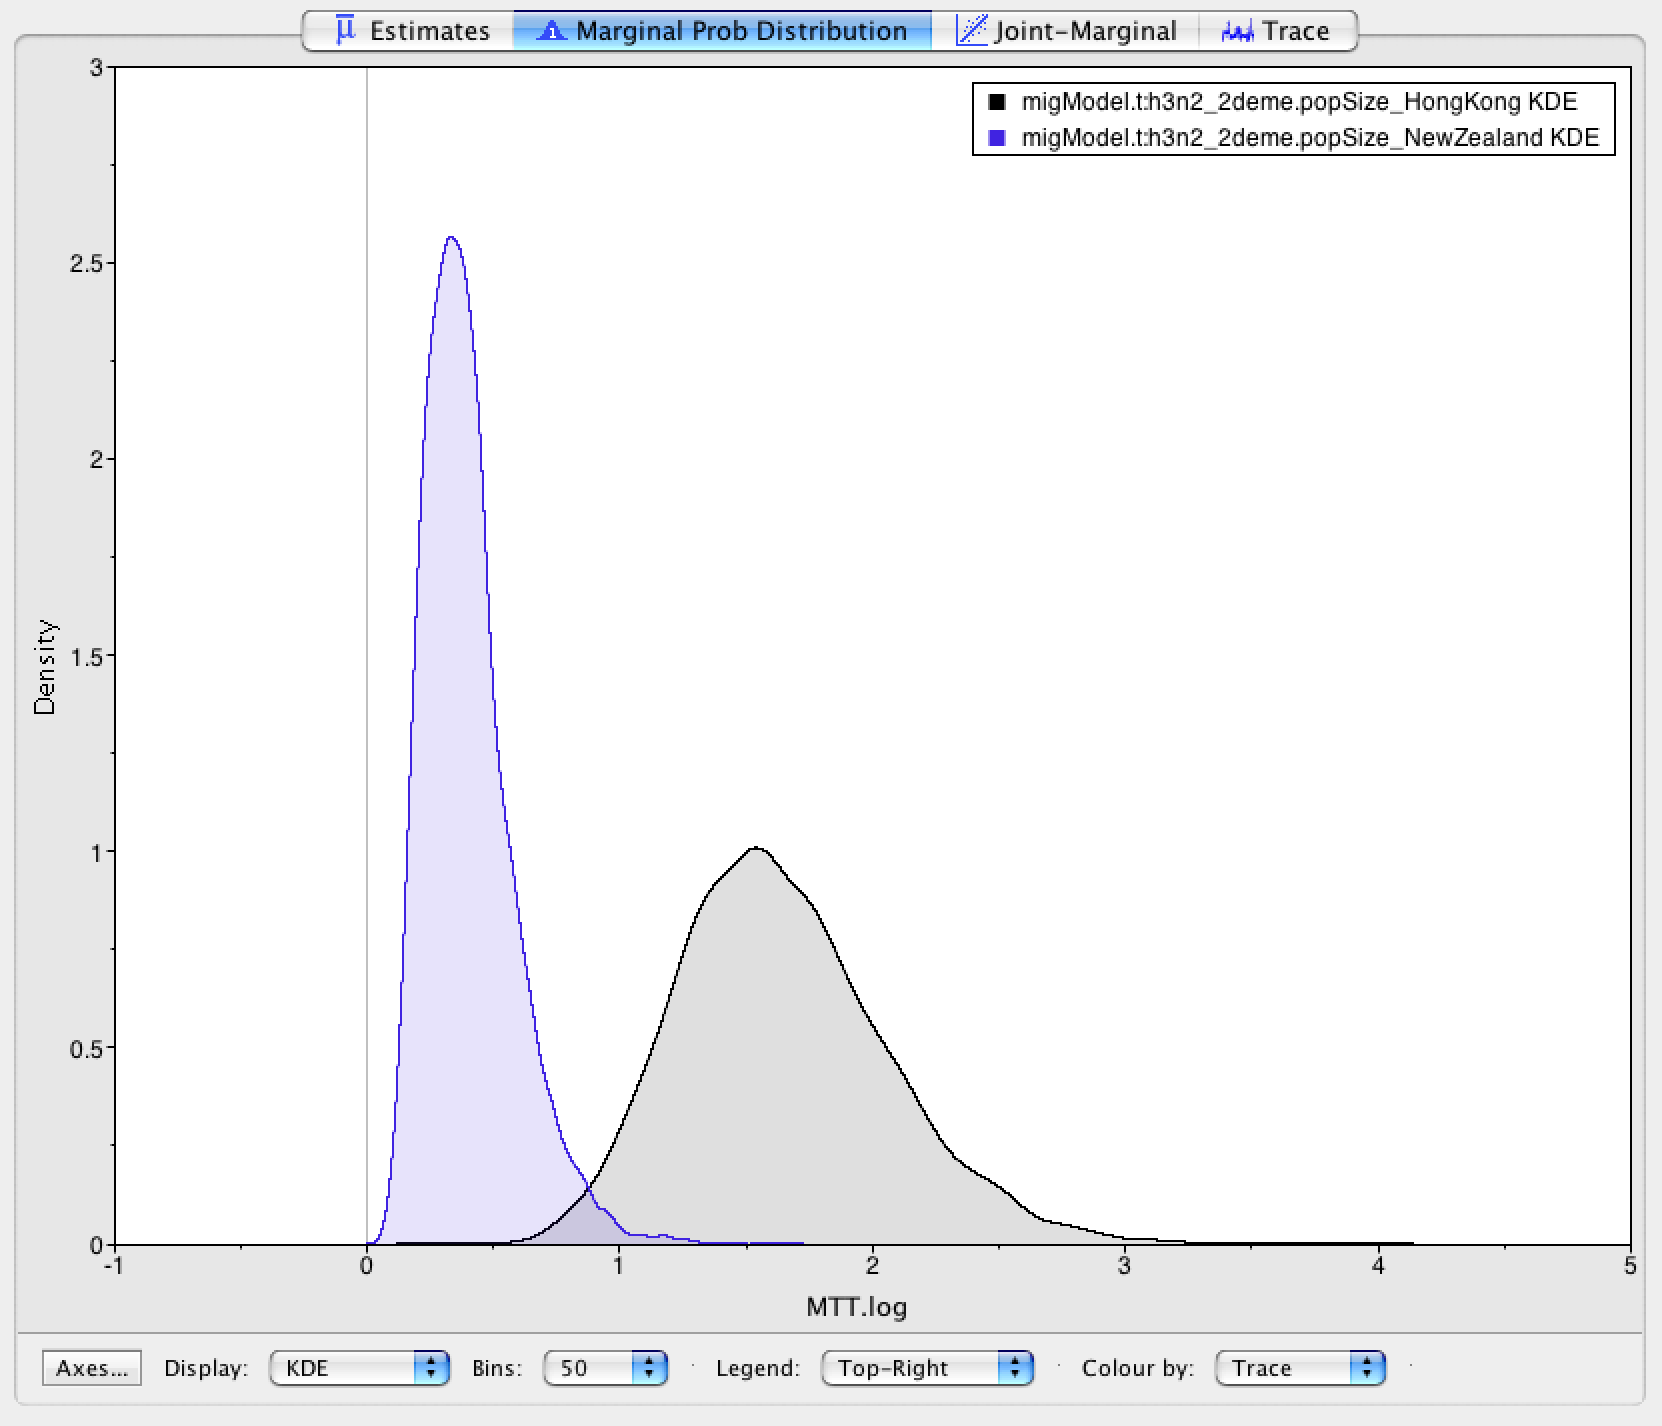
\includegraphics[width=0.600000\textwidth]{figures/effectivePsize_tracer.png}
    \caption{Estimated effective population sizes.}
    \label{fig:estimated_peff}
\end{figure}

Hong Kong ($ \sim $7 Mio Inhabitants) is inferred to have
the larger effective population size than New Zealand
($ \sim $ 4.5 Mio Inhabitants). Keep in mind though that the
effective population size is not only dependent on the population size
itself, but also on e.g.~transmission rates or contact rates.
Differences in the real population size are therefore not necessarily
reflected in the effective population size. However, they can still act
as a sanity test. Next, we want to have a look at the inferred migration
rates (Figure \protect\hyperlink{fig:etimated_mig}{7}).

\begin{figure}
    \centering
    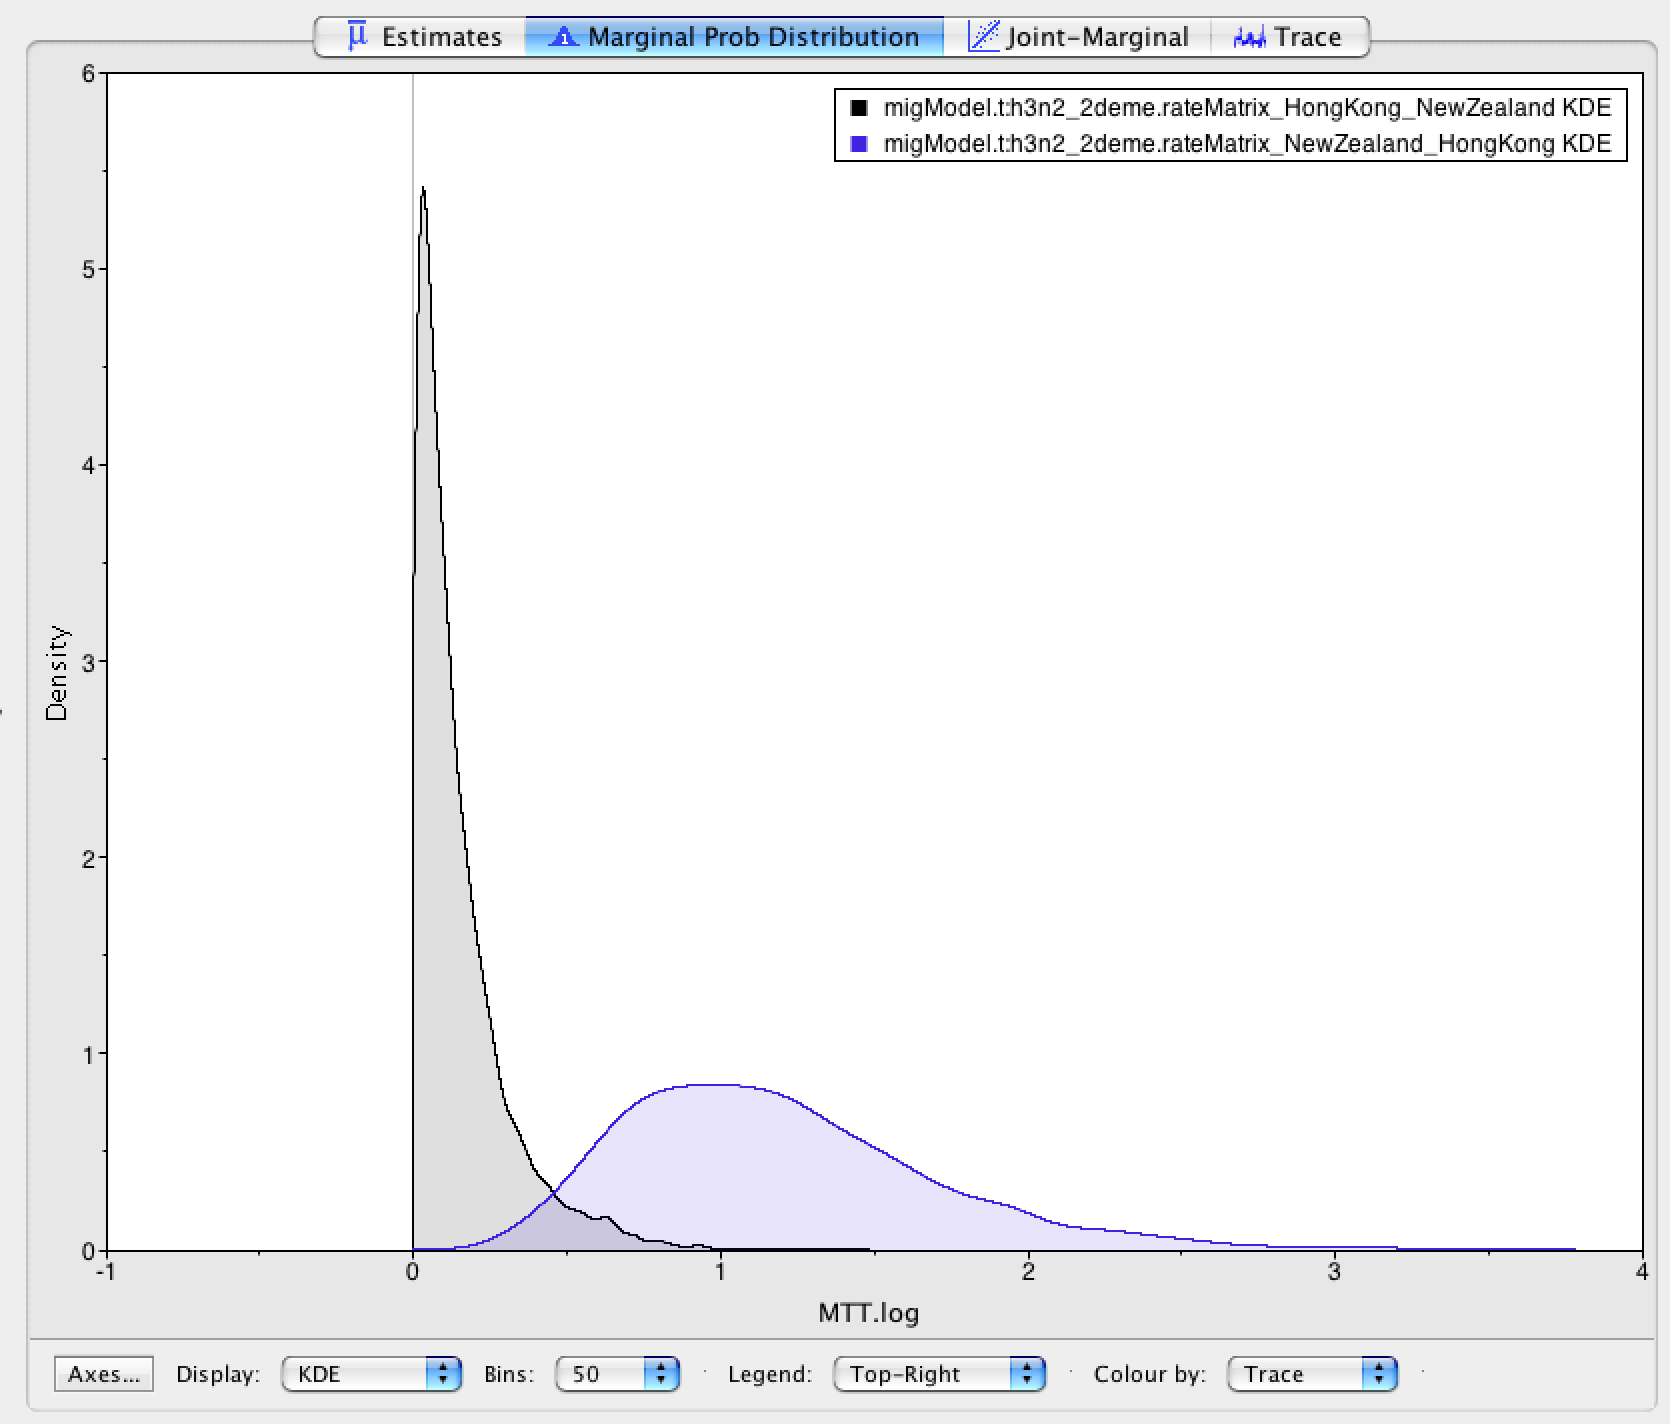
\includegraphics[width=0.600000\textwidth]{figures/migrationrates_tracer.png}
    \caption{Estimated migration rates.}
    \label{fig:etimated_mig}
\end{figure}

 \clearpage

As we stated at the beginning, it is assumed that South-East Asia works
as a global source of influenza, while e.g.~Oceania acts as a sink.

\begin{framed}
Do the inferred migration rates agree with this hypothesis?
\end{framed}

After having looked at the inferred parameters, we can look at the
inferred trees. We can either look at all the sampled trees individually
or can use a summary of all tree. This can be done by using the program
TreeAnnotator:

\begin{framed}
We need to specify at least 4 settings there. First, the burn-in
percentage, then the input tree file, the output tree file for which we
have to specify a file name and the \lstinline!Node Heights! (set it to
\lstinline!Mean Heights!)
\end{framed}

MultiTypeTree logs 3 different tree files:

\begin{itemize}

\item
  The first one is the \lstinline!*.map.trees! file. It contains the
  maximum posterior tree for the analysis up to a sample of the MCMC.
  This tree is the tree with the highest posterior probability that has
  been visited so far.
\item
  The second one is the \lstinline!*.trees! file. It contains the logged
  trees with so called single child node. In a normal tree, all nodes
  have two (or sometimes more) children. The nodes there are coalescent
  events. The single child nodes on the other hand are migration events
  (in this case a migration event between Hong Kong and New Zealand).
  MultiTypeTree infers the timing of those migration events on a branch
  and logs them in the \lstinline!*.trees! file.
\item
  The third tree file logged is the \lstinline!*.typedNode.trees!. This
  file does not use single child nodes. Instead, every coalescent event
  (here always a node with two daughter lineages) has a location (or
  state or color or type) where it was inferred to take place (see
  Figure \protect\hyperlink{fig:single_child}{8})
\end{itemize}

\begin{figure}
    \centering
    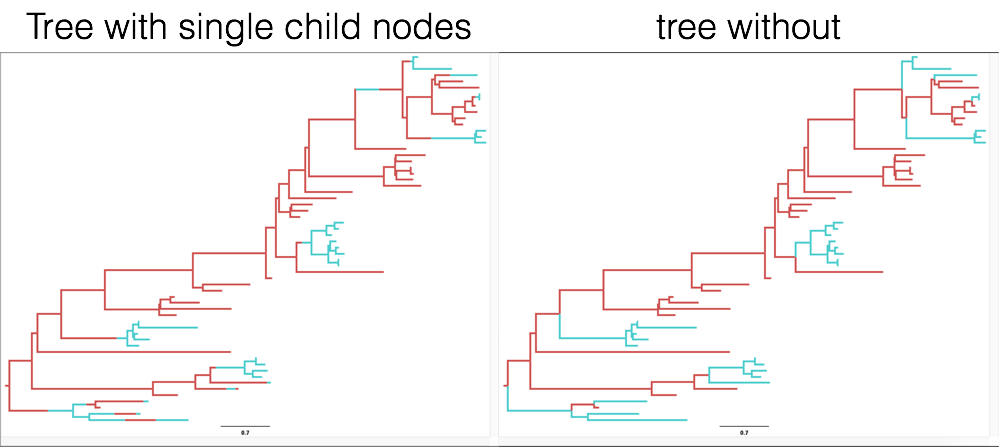
\includegraphics[max width=\textwidth, max height=0.9\textheight]{figures/single_child.png}
    \caption{An example of a tree where the migration events are logged as single child nodes (left) and of the same tree where only the location of a coalescent event is logged (right).}
    \label{fig:single_child}
\end{figure}

To summarize all the trees, we will need the
\lstinline!*.typedNode.trees! files, since TreeAnnotator cannot handle
single child nodes. We will also need to specify the \textbf{Burnin
percentage}, which we can guess from looking at the traces of the
parameter estimates in Tracer (10\% should be more than enough). Next,
we also need to specify where the output will be saved and under what
name. After that, we can run the analysis.

When TreeAnnotator is finished, we can visualize the summarized
MultiTypeTree run with FigTree.

\begin{framed}
Open the program and go to \lstinline!File > Open!, and open the output
tree file from TreeAnnotator.

To color the tree, go to \textbf{Appearance} and change \textbf{Colour
by} and \textbf{Width by}.

To get the coloring by inferred location, one has to set it to
\textbf{type}. The expressions \textbf{type, state, location and color}
are often used interchangeably. The color gives the estimated (most
likely) location of a node (red for Hong Kong and blue for New Zealand),
the width gives the certainty of a color. The more certain the estimate
is, the wider the branch above (towards the root of) the node. You can
also change the \textbf{Line Weight} to better see difference in the
width of branches.
\end{framed}

\begin{figure}
    \centering
    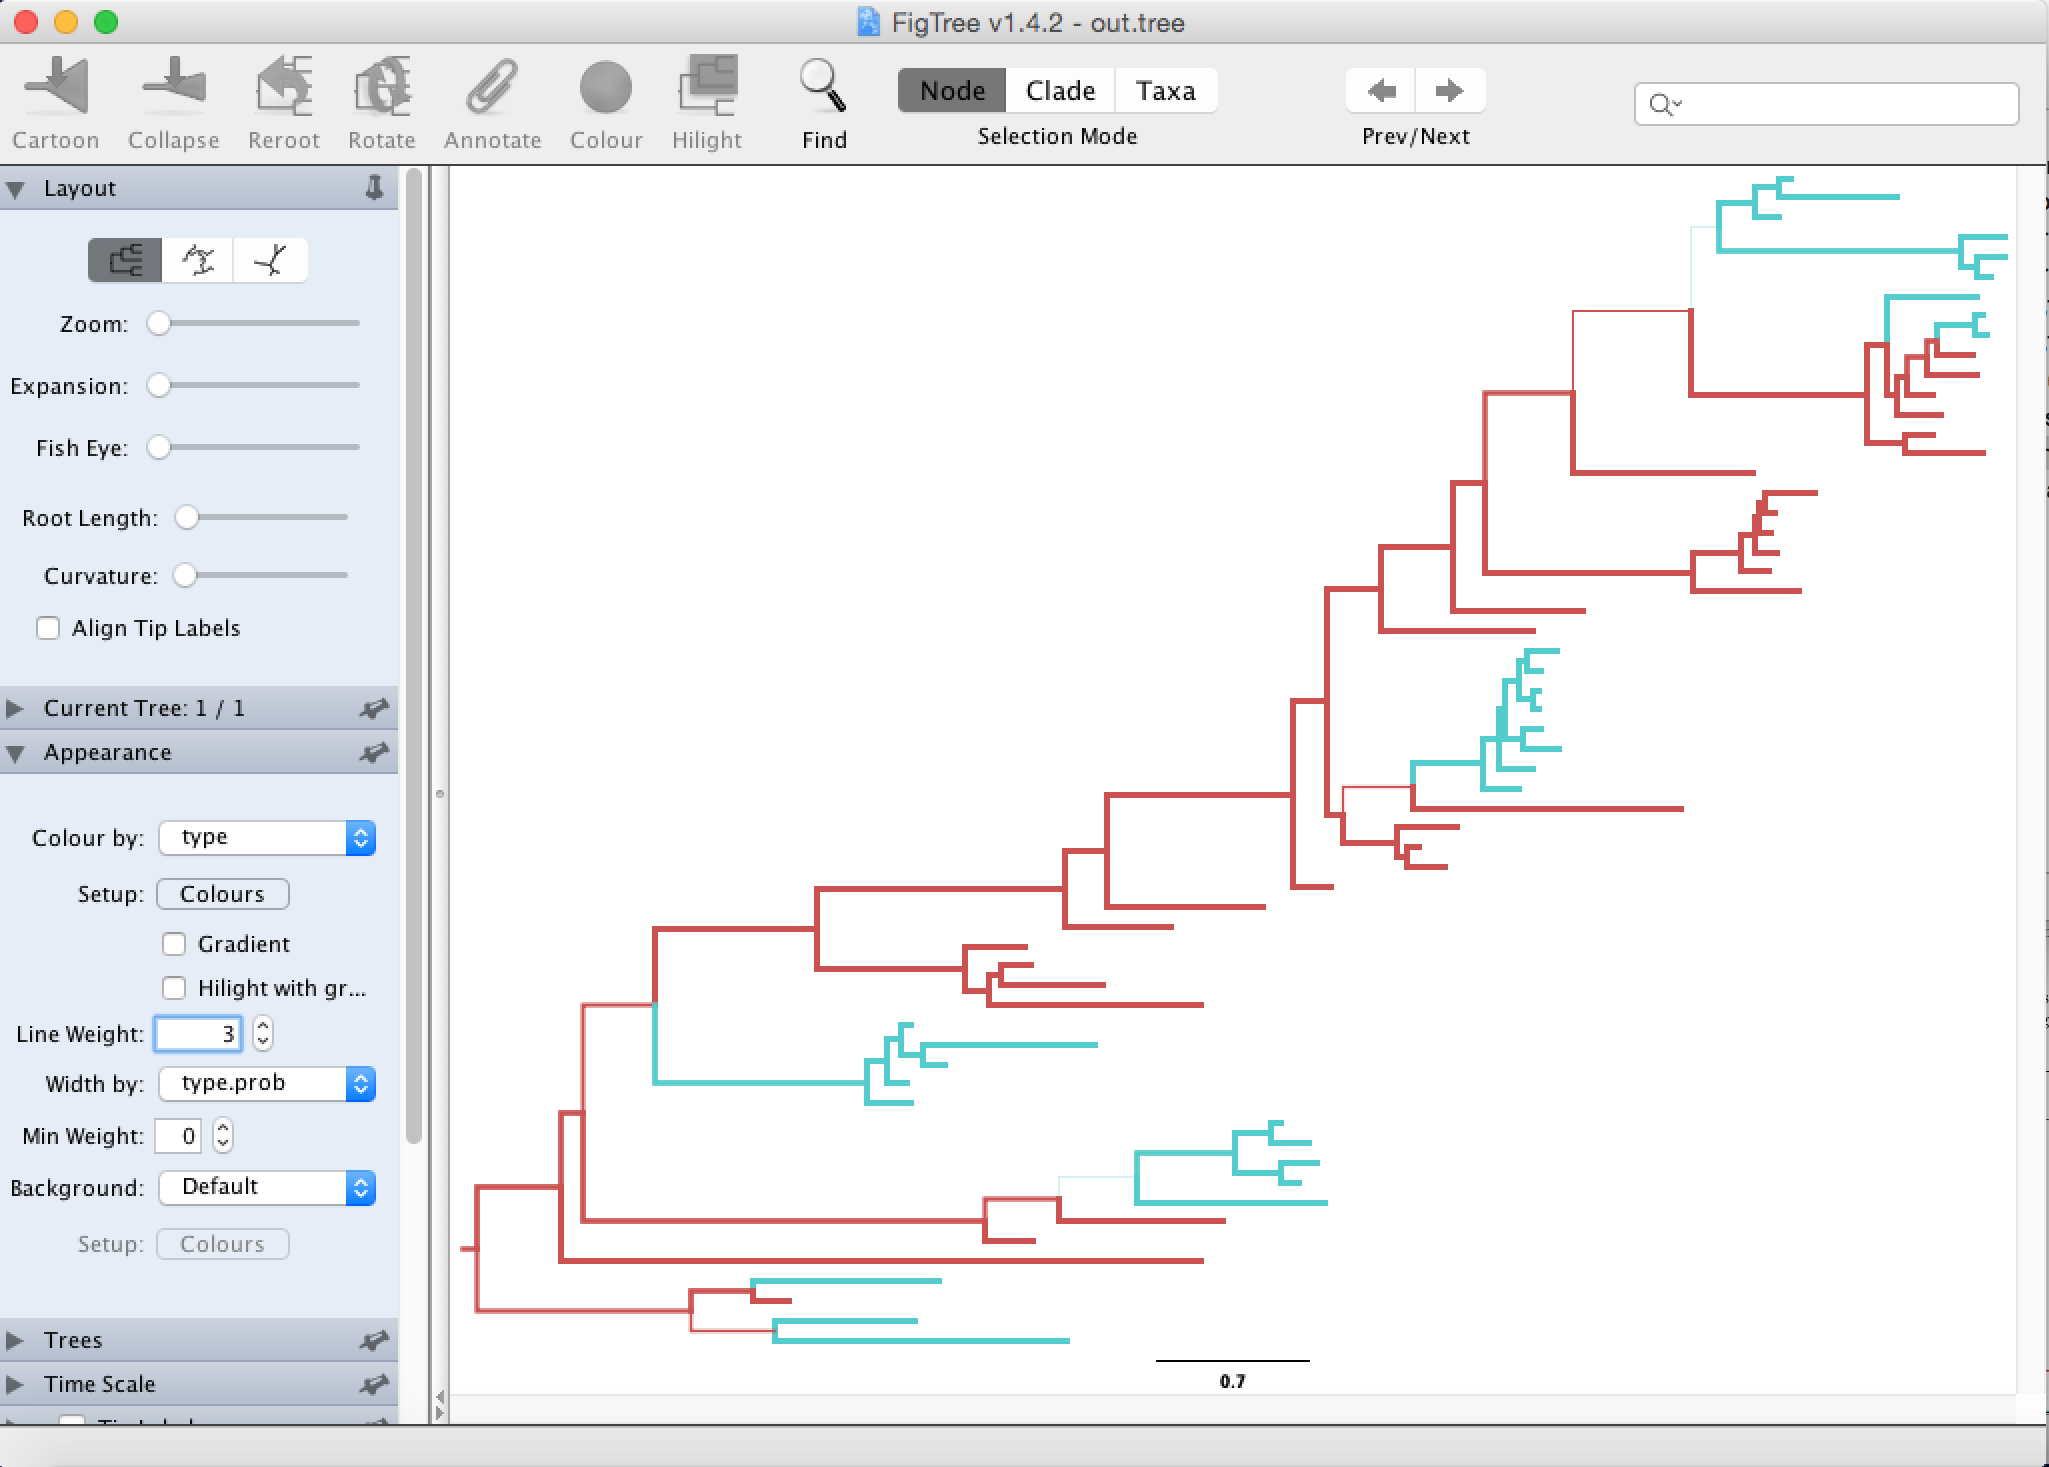
\includegraphics[max width=\textwidth, max height=0.9\textheight]{figures/figtree_color.png}
    \caption{Color tree according to the inferred location.}
    \label{fig:example}
\end{figure}

Next, we would like to know how certain we are about the node heights.

\begin{framed}
This can be visualized by going to \textbf{Node Bars} and there
\textbf{Display} the 95\% HPD of node heights, which gives the 95\%
credibility interval of node heights (the mean is indicated by the shown
node height).
\end{framed}

\begin{figure}
    \centering
    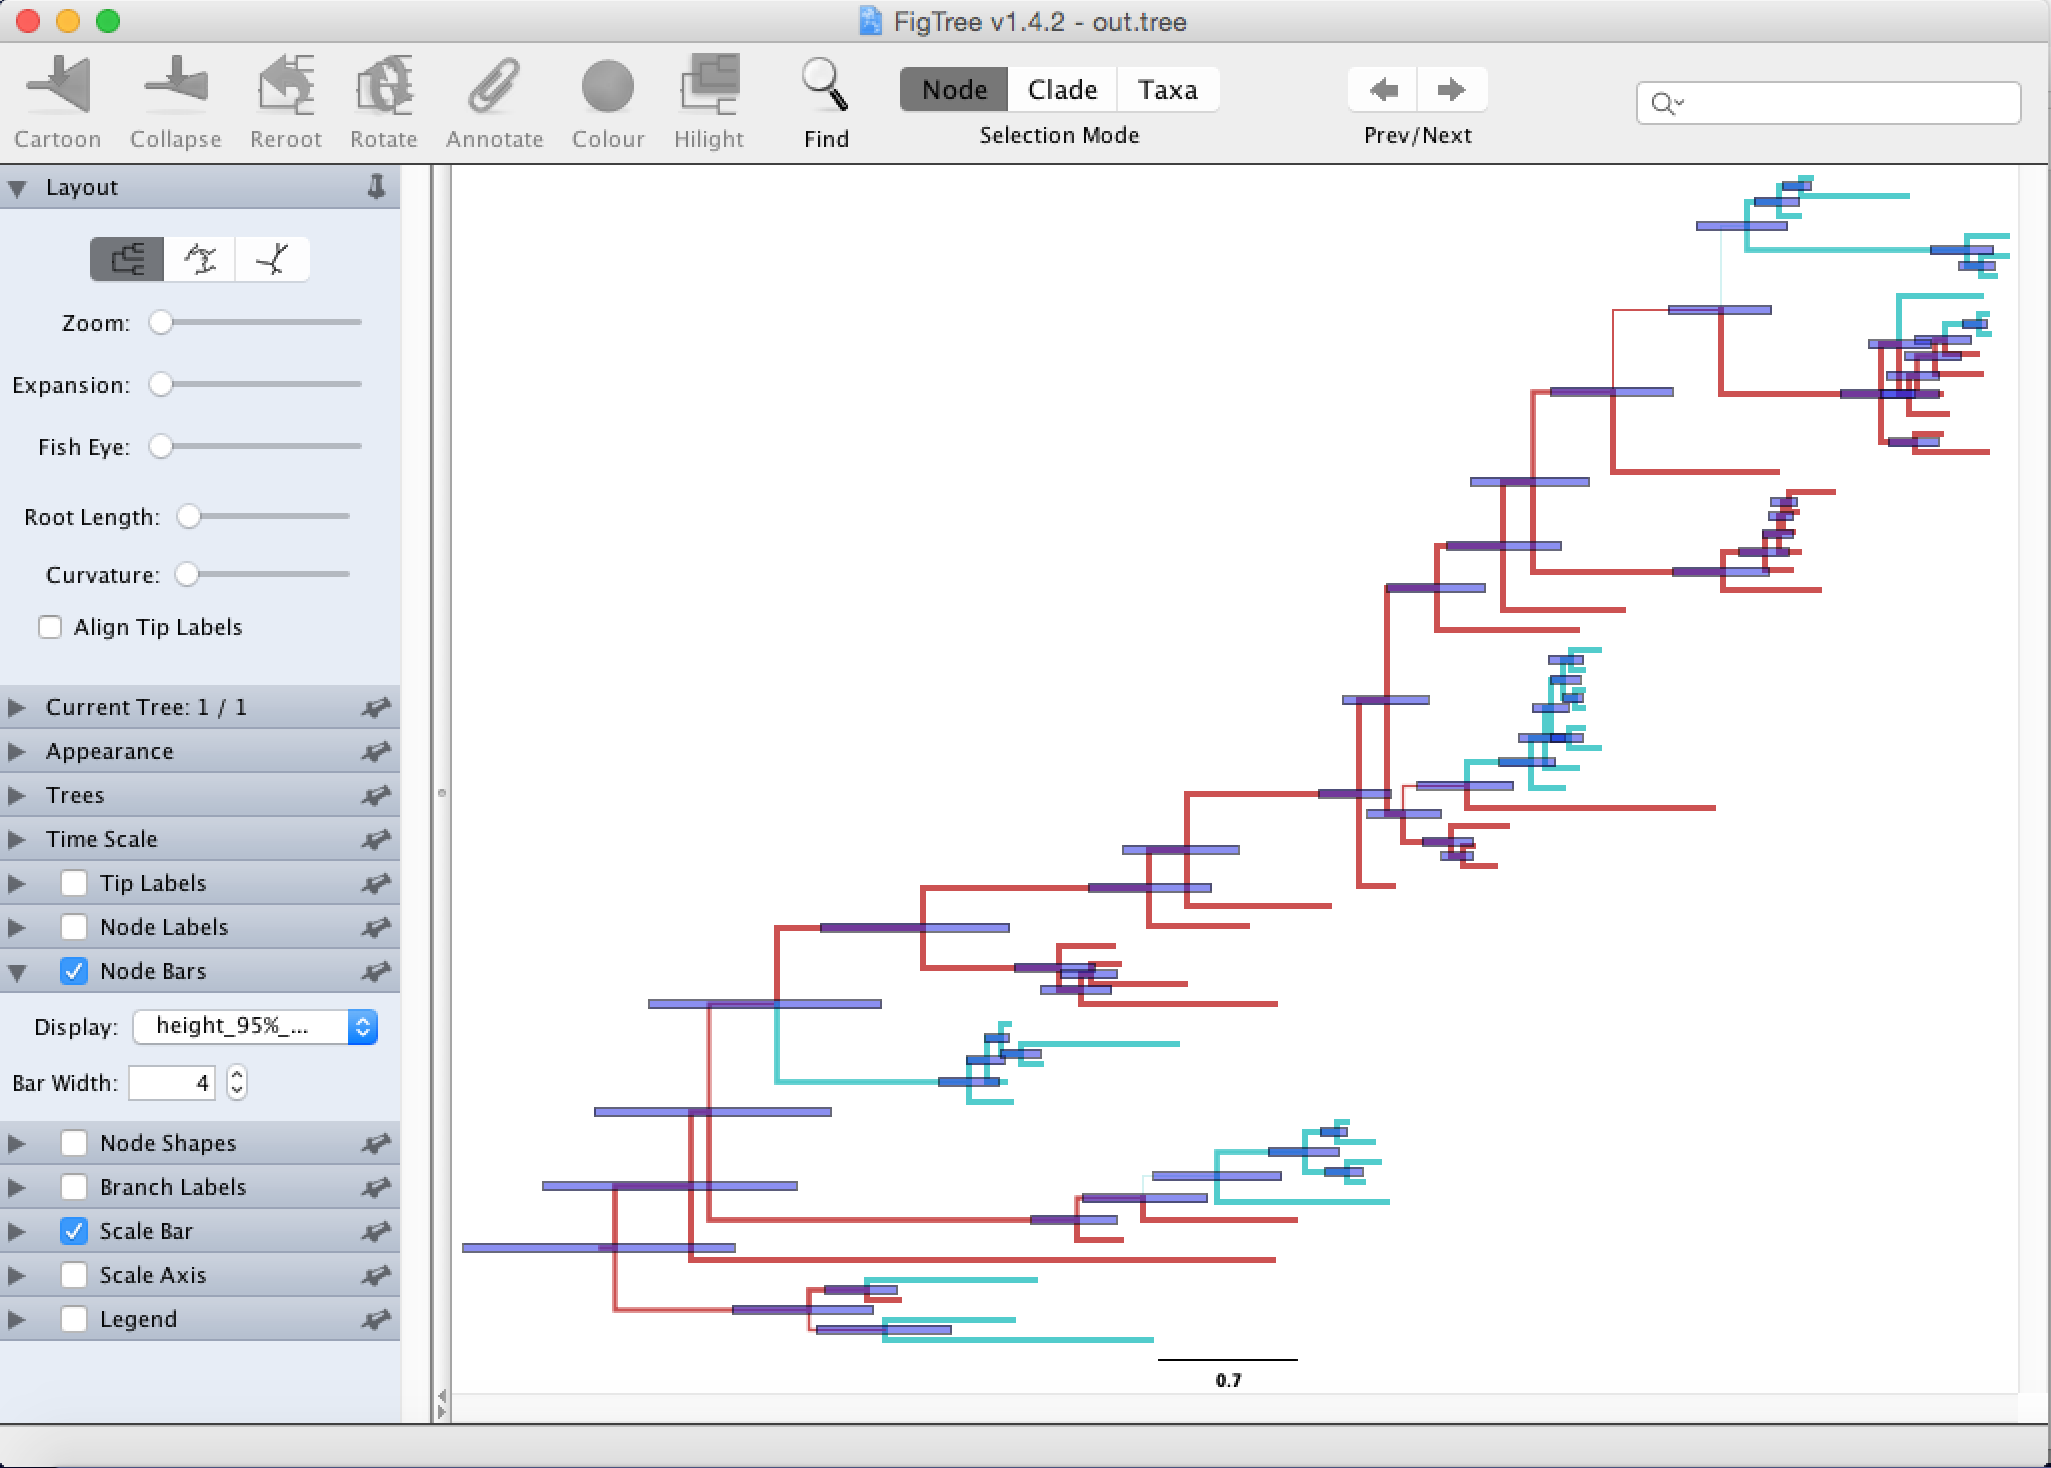
\includegraphics[max width=\textwidth, max height=0.9\textheight]{figures/figtree_nodeheights.png}
    \caption{Set the 95\% HPD for the node heights.}
    \label{fig:example}
\end{figure}

\subsubsection{Some considerations for using the structured Coalescent
(or any structured
method)}\label{some-considerations-for-using-the-structured-coalescent-or-any-structured-method}

\begin{itemize}

\item
  Inferring structure on a tree is hard and requires a lot of
  assumptions, e.g.~that the migration rates don't change over time or
  populations are constant.
\item
  The number of migration events on a tree might be very low, to infer a
  rate from such a low number of events can be very hard. In general, it
  is easier to infer rates within a region (here the effective
  population size) than it is to infer rates between them, as there are
  simply more events within than between regions.
\item
  Despite considering structure in a tree, there might still be states
  or locations etc. that were not sampled. Even if a node is inferred to
  be in a location with high certainty, the results could look
  completely different if samples from other locations would be
  considered as well.
\end{itemize}

\section{Useful Links}\label{useful-links}

\begin{itemize}

\item
  \href{http://www.beast2.org/book.html}{\emph{Bayesian Evolutionary
  Analysis with BEAST 2}} \citep{BEAST2book2014}
\item
  BEAST 2 website and documentation: \url{http://www.beast2.org/}
\item
  BEAST 1 website and documentation: \url{http://beast.bio.ed.ac.uk}
\item
  Join the BEAST user discussion:
  \url{http://groups.google.com/group/beast-users}
\end{itemize}

\clearpage

The content of this tutorial is based on the
\href{https://github.com/CompEvol/MultiTypeTree/wiki/Beginner's-Tutorial}{MultiTypeTree}
tutorial by Tim Vaughan. \clearpage



%%%%%%%%%%%%%%%%%%%%%%%
% Tutorial disclaimer %
%%%%%%%%%%%%%%%%%%%%%%%
% Please do not change the license
% Add the author names and relevant links
% Add any other aknowledgments here
\href{http://creativecommons.org/licenses/by/4.0/}{
\includegraphics[scale=0.8]{figures/ccby.pdf}} This tutorial was written by Nicola F. Müller and Tim Vaughan for \href{https://taming-the-beast.github.io}{Taming the BEAST} and is licensed under a \href{http://creativecommons.org/licenses/by/4.0/}{Creative Commons Attribution 4.0 International License}. 


%%%%%%%%%%%%%%%%%%%%
% Do NOT edit this %
%%%%%%%%%%%%%%%%%%%%
Version dated: \today



\newpage

%%%%%%%%%%%%%%%%
%  REFERENCES  %
%%%%%%%%%%%%%%%%

\printbibliography[heading=relevref]


\end{document}